
\documentclass[12pt]{article}
\usepackage{graphicx}
\usepackage{amsmath}
\usepackage{listings}
\usepackage{color}

\definecolor{dkgreen}{rgb}{0,0.6,0}
\definecolor{dkblue}{rgb}{0,0.0,0.6}
\definecolor{dkred}{rgb}{0.9,0.0,0.1}

\begin{document}

\lstset{language=Fortran,tabsize=4,numbers=left,numberstyle=\tiny,basicstyle=\ttfamily\small\color{dkblue},stringstyle=\ttfamily\color{blue},keywordstyle=\rmfamily\color{dkred}\bfseries\emph,backgroundcolor=\color{white},commentstyle=\color{dkgreen}}

\title{Horner's Method and Trigonometric Functions}
\author{Paul Fischer \\
Department of Physics\\
California State University Long Beach}
\date{\today }

\maketitle

\begin{abstract}

Horner's method is used to increase the efficiency associated with computing finite polynomials. We apply this scheme in a {\tt Fortran90} code that computes a finite number of terms from the Taylor series for sine and cosine. We plot these approximations using {\tt Plot2} in the domain {\tt x} $\in$ [-2$\pi$, 2$\pi$] against {\tt Fortran90}'s built-in {\tt sin} and {\tt cos} functions for different values of {\tt imax}, the highest degree of the Taylor series approximation. The errors associated with these computations are discussed qualitatively.

\end{abstract}

\section{Introduction}

Numerically approximating a function by calculating and adding each term of its Taylor series can be computationally intensive when trying to achieve a desired precision.  In 1819, British Mathematician William George Horner published a scheme for evaluating polynomials of degree {\tt n} with only {\tt n} additions and {\tt n} multiplications \cite{wiki}. This method is shown in Fig.\ \ref{horner}.  Section 2 will discuss our {\tt Fortran90} code that approximates the sine and cosine functions using Horner's method and will qualitatively evaluate the precision of the results of this method when plotted against the built-in {\tt Fortran90 sin} and {\tt cos} functions in the domain {\tt x} $\in$ [-2$\pi$, 2$\pi$] for different values of {\tt imax}, the highest degree of the Taylor series approximation. 

\begin{figure}[htb]
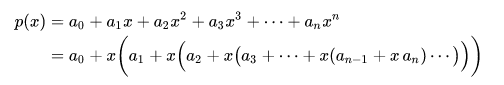
\includegraphics[width=1.\textwidth]{fig/horner.png}
\caption{Horner's method for finite polynomials \cite{wiki}.}
\label{horner}
\end{figure}

\section{Applying Horner's Method to the Sine and Cosine Taylor Series}

We write a {\tt Fortran90} code that uses Horner's method to approximate the sine and cosine functions from their Taylor series to a given degree {\tt imax}. The Makefile used for the code is shown in in Listing\ \ref{makefile}.

\begin{lstlisting}[frame=single,caption={{\tt Makefile}},label=makefile]

objs1 = numtype.o htrig.o

prog1 = htrig

f90 = gfortran

f90flags = -O3 

libs = -framework Accelerate

ldflags = $(libs)

all: $(prog1)

$(prog1): $(objs1)
	$(f90) $(ldflags) -o $@ $(objs1)

clean: 
	rm -f $(prog1) *.{o,mod} fort.*

.suffixes: $(suffixes) .f90

%.o: %.f90
	$(f90) $(f90flags) -c $<

\end{lstlisting}

The code is shown for sine and cosine in Listing\ \ref{htrigf90} for {\tt imax} = 100. The precision is defined in the Module {\tt numtype} shown in Listing\ \ref{module}. For each trigonometric function, the code uses a {\tt do} loop to create an array {\tt coeff} that contains the coefficients of the desired Taylor series up to the degree {\tt imax}.  Another {\tt do} loop writes to the files {\tt fort.1} (for sine) and {\tt fort.3} (for cosine) Horner's method approximations (contained in a nested {\tt do} loop) of the trigonometric functions against their corresponding {\tt x}-values in the domain {\tt x} $\in$ [-2$\pi$, 2$\pi$] separated by units of $\pi/30$. This {\tt do} loop also writes to the files {\tt fort.2} and {\tt fort.4} the same {\tt x}-values with their new corresponding {\tt y}-values given by the built-in {\tt sin} and {\tt cos} functions respectively.

\begin{lstlisting}[frame=single,caption={Module {\tt numtype}},label=module]

module numtype
    save
    integer, parameter :: dp = selected_real_kind(15,307)
    real(dp), parameter :: pi = 4*atan(1._dp)
    
end module numtype

\end{lstlisting}

\begin{lstlisting}[frame=single,caption={Program {\tt htrig.f90}},label=htrigf90]

program htrig

    use numtype
    implicit none

    real(dp) :: coeff(0:100)
    real(dp) :: x, y, dx
    integer :: i, imax

    ! Horner scheme for sine function

    imax = 100

    coeff(0) = 0
    coeff(1) = 1
    coeff(2:imax:2) = 0

    do i = 3, imax-1, 2
        coeff(i) = -coeff(i-2) / (i*(i-1))
    end do

    x = -2*pi
    dx = pi/30

    do while (x .le. 2*pi)
        y = coeff(imax)
        do i = imax-1, 0, -1
            y = coeff(i) + x*y 
        end do
        write(1,*) x, y
        y = sin(x)
        write(2,*) x, y
        x = x+dx
    end do 

    ! ---------------------------------
    
    ! Horner scheme for cosine function

    coeff(0) = 1
    coeff(1:imax:2) = 0

    do i = 2, imax, 2
        coeff(i) = -coeff(i-2) / (i*(i-1))
    end do

    x = -2*pi
    dx = pi/30

    do while (x .le. 2*pi)
        y = coeff(imax)
        do i = imax-1, 0, -1
        y = coeff(i) + x*y 
        end do
        write(3,*) x, y
        y = cos(x)
        write(4,*) x, y
        x = x+dx
    end do 

end program htrig

\end{lstlisting}


We can run the code by typing {\tt ./htrig}. The files {\tt fort.1} and {\tt fort.2} are plotted using {\tt Plot2} in Fig.\ \ref{sinimax10} with {\tt imax} = 10. This plot shows the large difference between the Horner's method approximation for sine and the built-in {\tt sin} function for such a small {\tt imax} value. The values for {\tt imax} were chosen in an effort to visually see the limit where the Horner's method plots start to coincide with the built-in function plots.  An {\tt imax} value of 16 was used in Fig.\ \ref{sinimax16}.  This value shows that the Horner approximation is rapidly converging to the built-in function within the interval but is still visually off at the ends.  It is hard to see any difference between the Horner's method approximation and the built-in function when {\tt imax} = 100 was used for Fig.\ \ref{sinimax100}.  The plot of the Horner approximation of the cosine function against the built-in {\tt cos} function for {\tt imax} = 100 is shown in Fig.\ \ref{cos}.

\begin{figure}[htb!]
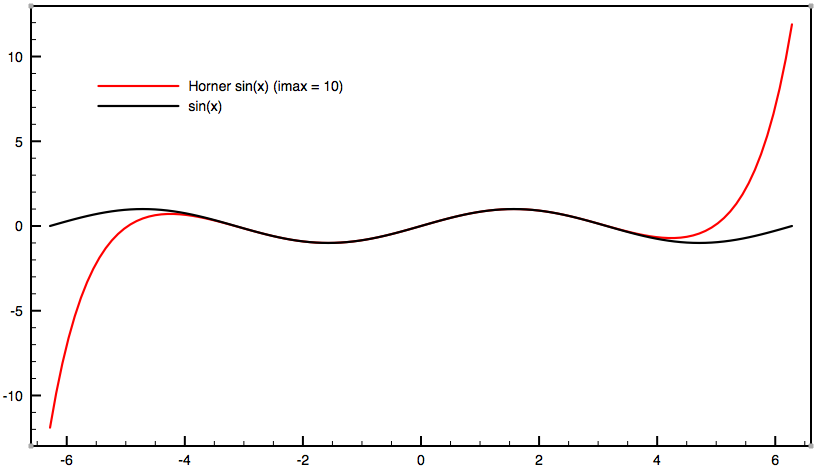
\includegraphics[width=1.\textwidth]{fig/sinimax10.png}
\caption{Horner sin vs. built-in {\tt sin} for {\tt x} $\in$ [-2$\pi$, 2$\pi$], {\tt imax} = 10.}
\label{sinimax10}
\end{figure}

\begin{figure}[htb!]
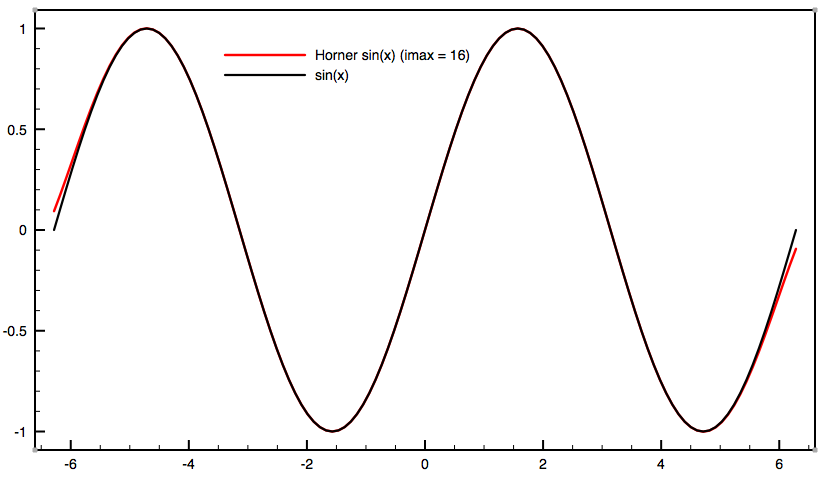
\includegraphics[width=1.\textwidth]{fig/sinimax16.png}
\caption{Horner sin vs. built-in {\tt sin} for {\tt x} $\in$ [-2$\pi$, 2$\pi$], {\tt imax} = 16.}
\label{sinimax16}
\end{figure}

\begin{figure}[htb!]
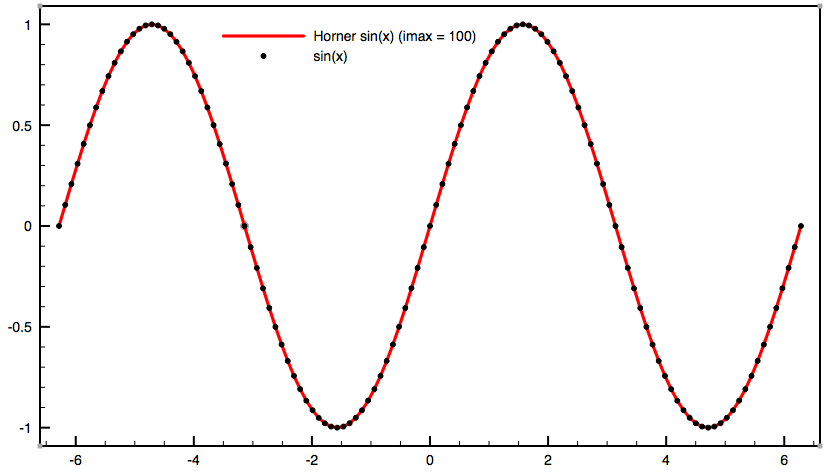
\includegraphics[width=1.\textwidth]{fig/sinimax100.png}
\caption{Horner sin vs. built-in {\tt sin} for {\tt x} $\in$ [-2$\pi$, 2$\pi$], {\tt imax} = 100.}
\label{sinimax100}
\end{figure}

\begin{figure}[htb!]
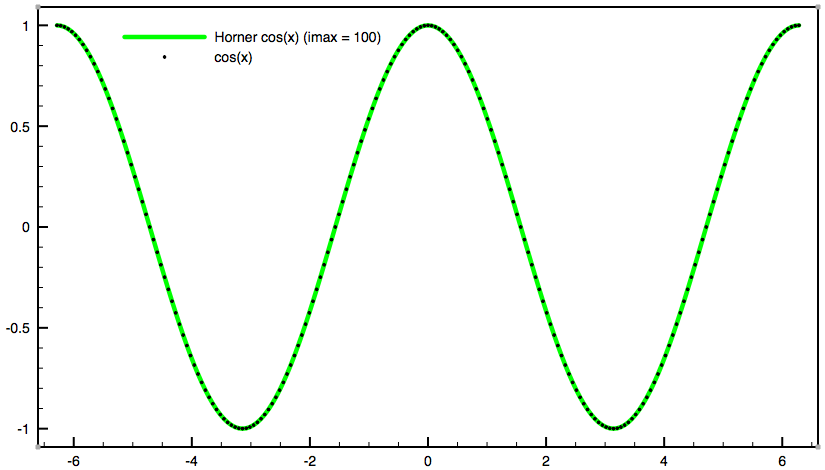
\includegraphics[width=1.\textwidth]{fig/cos.png}
\caption{Horner cos vs. built-in {\tt cos} for {\tt x} $\in$ [-2$\pi$, 2$\pi$], {\tt imax} = 100.}
\label{cos}
\end{figure}

\section{Summary and conclusions}

We presented our {\tt Fortran90} code for the Horner's method approximation of sine and cosine and qualitatively looked at the degrees {\tt imax} to which the approximation converges to the built-in functions. Horner's method allows for the calculation of these approximations to be done more efficiently than having the program add and multiply each term of the Taylor series separately. The plots indicate that at around 20 degrees the Horner approximation starts to be visually indistinguishable on the graph from the built-in functions.

\begin{thebibliography}{}

\bibitem{wiki} {\it Horner's Method} (n.d). In \emph{Wikipedia}. Retrieved January 30, 2020, https://en.wikipedia.org/wiki/Horner%27s_method

\end{thebibliography}

\end{document}
